\begin{frame}
    \begin{minipage}{0.45\textwidth}
        \textbf{\underline{First Approach} - Manual Feature Extraction}

        \vspace{0.5em}

        \begin{itemize}
            \item Simple \& fast to implement.
            \item Easy to interpret.
            \item Features might not be relevant.
            \item Difficulty in extracting some features. 
        \end{itemize}


    \end{minipage}%
    \hfill
    \begin{minipage}{0.45\textwidth}
        \centering
        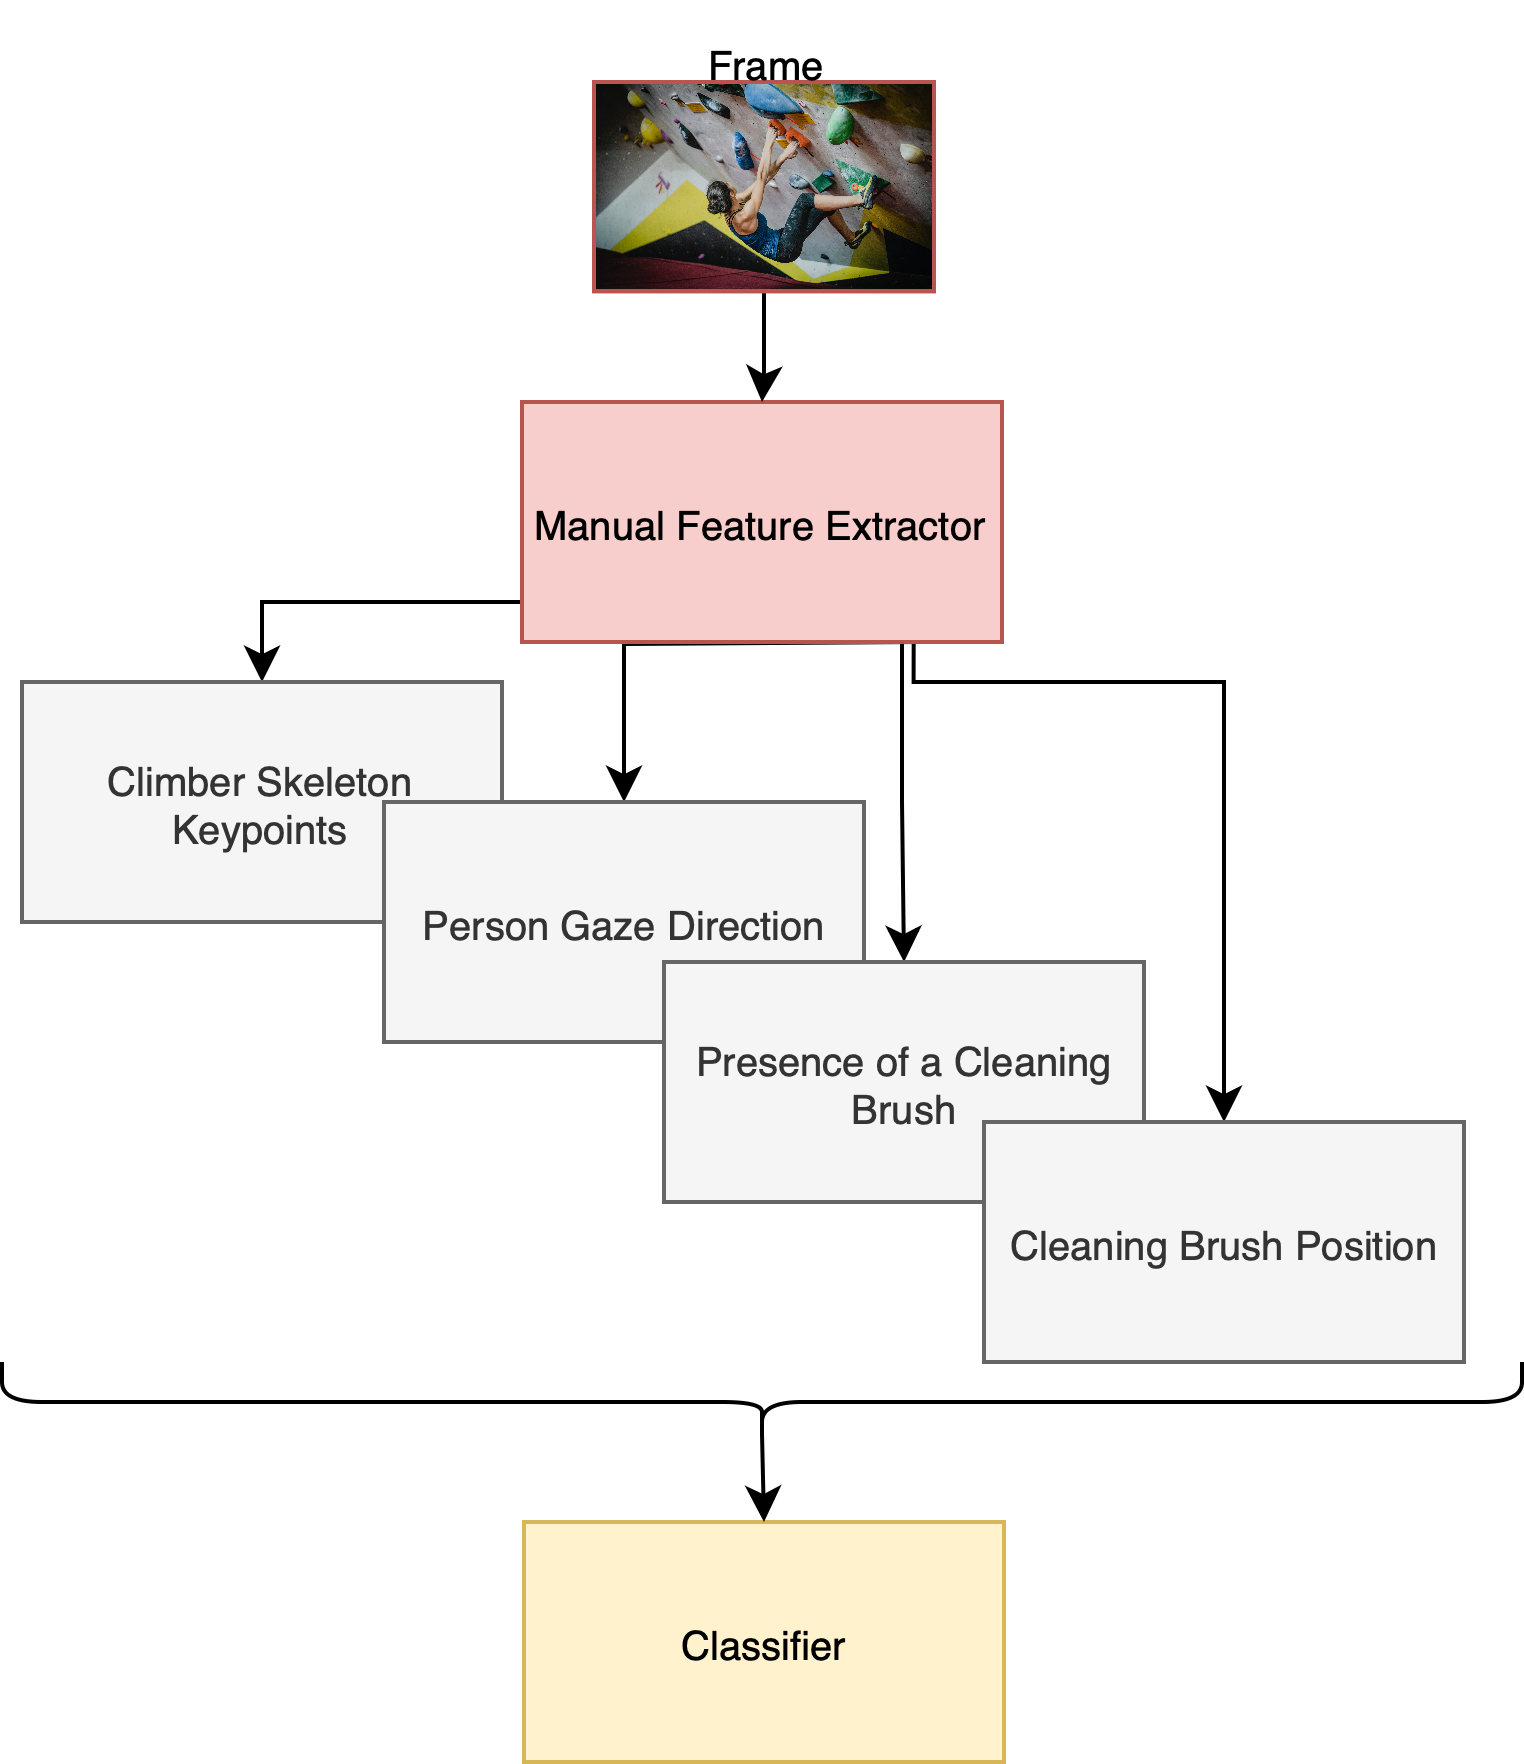
\includegraphics[width=0.9\textwidth]{assets/visuals/first-approach-visual.drawio.png} % Adjusted width
        
        % NOTE: during the talk justify and talk about the results we got
        % TODO: add a visual example of the segmentation results and say that there isn't so much zigzags in the talk
        % TODO: follow that with a visualization of PCA and say that to dig in more we tested visualization / clustering and found out that similar classes are grouped together ?
    \end{minipage}
\end{frame}


% To say during the discussion:
    % NOTE: specify when talking that the person's skeleton key points are relative to the center of it's body.
    % NOTE: a potential improvement for this approach is to track the different persons that are in the video and only focus on the one that stays the longest.
